
%% bare_conf.tex
%% V1.3
%% 2007/01/11
%% by Michael Shell
%% See:
%% http://www.michaelshell.org/
%% for current contact information.
%%
%% This is a skeleton file demonstrating the use of IEEEtran.cls
%% (requires IEEEtran.cls version 1.7 or later) with an IEEE conference paper.
%%
%% Support sites:
%% http://www.michaelshell.org/tex/ieeetran/
%% http://www.ctan.org/tex-archive/macros/latex/contrib/IEEEtran/
%% and
%% http://www.ieee.org/

%%*************************************************************************
%% Legal Notice:
%% This code is offered as-is without any warranty either expressed or
%% implied; without even the implied warranty of MERCHANTABILITY or
%% FITNESS FOR A PARTICULAR PURPOSE!
%% User assumes all risk.
%% In no event shall IEEE or any contributor to this code be liable for
%% any damages or losses, including, but not limited to, incidental,
%% consequential, or any other damages, resulting from the use or misuse
%% of any information contained here.
%%
%% All comments are the opinions of their respective authors and are not
%% necessarily endorsed by the IEEE.
%%
%% This work is distributed under the LaTeX Project Public License (LPPL)
%% ( http://www.latex-project.org/ ) version 1.3, and may be freely used,
%% distributed and modified. A copy of the LPPL, version 1.3, is included
%% in the base LaTeX documentation of all distributions of LaTeX released
%% 2003/12/01 or later.
%% Retain all contribution notices and credits.
%% ** Modified files should be clearly indicated as such, including  **
%% ** renaming them and changing author support contact information. **
%%
%% File list of work: IEEEtran.cls, IEEEtran_HOWTO.pdf, bare_adv.tex,
%%                    bare_conf.tex, bare_jrnl.tex, bare_jrnl_compsoc.tex
%%*************************************************************************

% *** Authors should verify (and, if needed, correct) their LaTeX system  ***
% *** with the testflow diagnostic prior to trusting their LaTeX platform ***
% *** with production work. IEEE's font choices can trigger bugs that do  ***
% *** not appear when using other class files.                            ***
% The testflow support page is at:
% http://www.michaelshell.org/tex/testflow/



% Note that the a4paper option is mainly intended so that authors in
% countries using A4 can easily print to A4 and see how their papers will
% look in print - the typesetting of the document will not typically be
% affected with changes in paper size (but the bottom and side margins will).
% Use the testflow package mentioned above to verify correct handling of
% both paper sizes by the user's LaTeX system.
%
% Also note that the "draftcls" or "draftclsnofoot", not "draft", option
% should be used if it is desired that the figures are to be displayed in
% draft mode.
%
\documentclass[conference]{IEEEtran}
% Add the compsoc option for Computer Society conferences.
%
% If IEEEtran.cls has not been installed into the LaTeX system files,
% manually specify the path to it like:
% \documentclass[conference]{../sty/IEEEtran}





% Some very useful LaTeX packages include:
% (uncomment the ones you want to load)


% *** MISC UTILITY PACKAGES ***
%
%\usepackage{ifpdf}
% Heiko Oberdiek's ifpdf.sty is very useful if you need conditional
% compilation based on whether the output is pdf or dvi.
% usage:
% \ifpdf
%   % pdf code
% \else
%   % dvi code
% \fi
% The latest version of ifpdf.sty can be obtained from:
% http://www.ctan.org/tex-archive/macros/latex/contrib/oberdiek/
% Also, note that IEEEtran.cls V1.7 and later provides a builtin
% \ifCLASSINFOpdf conditional that works the same way.
% When switching from latex to pdflatex and vice-versa, the compiler may
% have to be run twice to clear warning/error messages.






% *** CITATION PACKAGES ***
%
%\usepackage{cite}
% cite.sty was written by Donald Arseneau
% V1.6 and later of IEEEtran pre-defines the format of the cite.sty package
% \cite{} output to follow that of IEEE. Loading the cite package will
% result in citation numbers being automatically sorted and properly
% "compressed/ranged". e.g., [1], [9], [2], [7], [5], [6] without using
% cite.sty will become [1], [2], [5]--[7], [9] using cite.sty. cite.sty's
% \cite will automatically add leading space, if needed. Use cite.sty's
% noadjust option (cite.sty V3.8 and later) if you want to turn this off.
% cite.sty is already installed on most LaTeX systems. Be sure and use
% version 4.0 (2003-05-27) and later if using hyperref.sty. cite.sty does
% not currently provide for hyperlinked citations.
% The latest version can be obtained at:
% http://www.ctan.org/tex-archive/macros/latex/contrib/cite/
% The documentation is contained in the cite.sty file itself.






% *** GRAPHICS RELATED PACKAGES ***
%
\ifCLASSINFOpdf
  % \usepackage[pdftex]{graphicx}
  % declare the path(s) where your graphic files are
  % \graphicspath{{../pdf/}{../jpeg/}}
  % and their extensions so you won't have to specify these with
  % every instance of \includegraphics
  % \DeclareGraphicsExtensions{.pdf,.jpeg,.png}
\else
  % or other class option (dvipsone, dvipdf, if not using dvips). graphicx
  % will default to the driver specified in the system graphics.cfg if no
  % driver is specified.
  % \usepackage[dvips]{graphicx}
  % declare the path(s) where your graphic files are
  % \graphicspath{{../eps/}}
  % and their extensions so you won't have to specify these with
  % every instance of \includegraphics
  % \DeclareGraphicsExtensions{.eps}
\fi
% graphicx was written by David Carlisle and Sebastian Rahtz. It is
% required if you want graphics, photos, etc. graphicx.sty is already
% installed on most LaTeX systems. The latest version and documentation can
% be obtained at:
% http://www.ctan.org/tex-archive/macros/latex/required/graphics/
% Another good source of documentation is "Using Imported Graphics in
% LaTeX2e" by Keith Reckdahl which can be found as epslatex.ps or
% epslatex.pdf at: http://www.ctan.org/tex-archive/info/
%
% latex, and pdflatex in dvi mode, support graphics in encapsulated
% postscript (.eps) format. pdflatex in pdf mode supports graphics
% in .pdf, .jpeg, .png and .mps (metapost) formats. Users should ensure
% that all non-photo figures use a vector format (.eps, .pdf, .mps) and
% not a bitmapped formats (.jpeg, .png). IEEE frowns on bitmapped formats
% which can result in "jaggedy"/blurry rendering of lines and letters as
% well as large increases in file sizes.
%
% You can find documentation about the pdfTeX application at:
% http://www.tug.org/applications/pdftex





% *** MATH PACKAGES ***
%
%\usepackage[cmex10]{amsmath}
% A popular package from the American Mathematical Society that provides
% many useful and powerful commands for dealing with mathematics. If using
% it, be sure to load this package with the cmex10 option to ensure that
% only type 1 fonts will utilized at all point sizes. Without this option,
% it is possible that some math symbols, particularly those within
% footnotes, will be rendered in bitmap form which will result in a
% document that can not be IEEE Xplore compliant!
%
% Also, note that the amsmath package sets \interdisplaylinepenalty to 10000
% thus preventing page breaks from occurring within multiline equations. Use:
%\interdisplaylinepenalty=2500
% after loading amsmath to restore such page breaks as IEEEtran.cls normally
% does. amsmath.sty is already installed on most LaTeX systems. The latest
% version and documentation can be obtained at:
% http://www.ctan.org/tex-archive/macros/latex/required/amslatex/math/





% *** SPECIALIZED LIST PACKAGES ***
%
%\usepackage{algorithmic}
% algorithmic.sty was written by Peter Williams and Rogerio Brito.
% This package provides an algorithmic environment fo describing algorithms.
% You can use the algorithmic environment in-text or within a figure
% environment to provide for a floating algorithm. Do NOT use the algorithm
% floating environment provided by algorithm.sty (by the same authors) or
% algorithm2e.sty (by Christophe Fiorio) as IEEE does not use dedicated
% algorithm float types and packages that provide these will not provide
% correct IEEE style captions. The latest version and documentation of
% algorithmic.sty can be obtained at:
% http://www.ctan.org/tex-archive/macros/latex/contrib/algorithms/
% There is also a support site at:
% http://algorithms.berlios.de/index.html
% Also of interest may be the (relatively newer and more customizable)
% algorithmicx.sty package by Szasz Janos:
% http://www.ctan.org/tex-archive/macros/latex/contrib/algorithmicx/




% *** ALIGNMENT PACKAGES ***
%
%\usepackage{array}
% Frank Mittelbach's and David Carlisle's array.sty patches and improves
% the standard LaTeX2e array and tabular environments to provide better
% appearance and additional user controls. As the default LaTeX2e table
% generation code is lacking to the point of almost being broken with
% respect to the quality of the end results, all users are strongly
% advised to use an enhanced (at the very least that provided by array.sty)
% set of table tools. array.sty is already installed on most systems. The
% latest version and documentation can be obtained at:
% http://www.ctan.org/tex-archive/macros/latex/required/tools/


%\usepackage{mdwmath}
%\usepackage{mdwtab}
% Also highly recommended is Mark Wooding's extremely powerful MDW tools,
% especially mdwmath.sty and mdwtab.sty which are used to format equations
% and tables, respectively. The MDWtools set is already installed on most
% LaTeX systems. The lastest version and documentation is available at:
% http://www.ctan.org/tex-archive/macros/latex/contrib/mdwtools/


% IEEEtran contains the IEEEeqnarray family of commands that can be used to
% generate multiline equations as well as matrices, tables, etc., of high
% quality.


%\usepackage{eqparbox}
% Also of notable interest is Scott Pakin's eqparbox package for creating
% (automatically sized) equal width boxes - aka "natural width parboxes".
% Available at:
% http://www.ctan.org/tex-archive/macros/latex/contrib/eqparbox/





% *** SUBFIGURE PACKAGES ***
%\usepackage[tight,footnotesize]{subfigure}
% subfigure.sty was written by Steven Douglas Cochran. This package makes it
% easy to put subfigures in your figures. e.g., "Figure 1a and 1b". For IEEE
% work, it is a good idea to load it with the tight package option to reduce
% the amount of white space around the subfigures. subfigure.sty is already
% installed on most LaTeX systems. The latest version and documentation can
% be obtained at:
% http://www.ctan.org/tex-archive/obsolete/macros/latex/contrib/subfigure/
% subfigure.sty has been superceeded by subfig.sty.



%\usepackage[caption=false]{caption}
%\usepackage[font=footnotesize]{subfig}
% subfig.sty, also written by Steven Douglas Cochran, is the modern
% replacement for subfigure.sty. However, subfig.sty requires and
% automatically loads Axel Sommerfeldt's caption.sty which will override
% IEEEtran.cls handling of captions and this will result in nonIEEE style
% figure/table captions. To prevent this problem, be sure and preload
% caption.sty with its "caption=false" package option. This is will preserve
% IEEEtran.cls handing of captions. Version 1.3 (2005/06/28) and later
% (recommended due to many improvements over 1.2) of subfig.sty supports
% the caption=false option directly:
%\usepackage[caption=false,font=footnotesize]{subfig}
%
% The latest version and documentation can be obtained at:
% http://www.ctan.org/tex-archive/macros/latex/contrib/subfig/
% The latest version and documentation of caption.sty can be obtained at:
% http://www.ctan.org/tex-archive/macros/latex/contrib/caption/




% *** FLOAT PACKAGES ***
%
%\usepackage{fixltx2e}
% fixltx2e, the successor to the earlier fix2col.sty, was written by
% Frank Mittelbach and David Carlisle. This package corrects a few problems
% in the LaTeX2e kernel, the most notable of which is that in current
% LaTeX2e releases, the ordering of single and double column floats is not
% guaranteed to be preserved. Thus, an unpatched LaTeX2e can allow a
% single column figure to be placed prior to an earlier double column
% figure. The latest version and documentation can be found at:
% http://www.ctan.org/tex-archive/macros/latex/base/



%\usepackage{stfloats}
% stfloats.sty was written by Sigitas Tolusis. This package gives LaTeX2e
% the ability to do double column floats at the bottom of the page as well
% as the top. (e.g., "\begin{figure*}[!b]" is not normally possible in
% LaTeX2e). It also provides a command:
%\fnbelowfloat
% to enable the placement of footnotes below bottom floats (the standard
% LaTeX2e kernel puts them above bottom floats). This is an invasive package
% which rewrites many portions of the LaTeX2e float routines. It may not work
% with other packages that modify the LaTeX2e float routines. The latest
% version and documentation can be obtained at:
% http://www.ctan.org/tex-archive/macros/latex/contrib/sttools/
% Documentation is contained in the stfloats.sty comments as well as in the
% presfull.pdf file. Do not use the stfloats baselinefloat ability as IEEE
% does not allow \baselineskip to stretch. Authors submitting work to the
% IEEE should note that IEEE rarely uses double column equations and
% that authors should try to avoid such use. Do not be tempted to use the
% cuted.sty or midfloat.sty packages (also by Sigitas Tolusis) as IEEE does
% not format its papers in such ways.





% *** PDF, URL AND HYPERLINK PACKAGES ***
%
%\usepackage{url}
% url.sty was written by Donald Arseneau. It provides better support for
% handling and breaking URLs. url.sty is already installed on most LaTeX
% systems. The latest version can be obtained at:
% http://www.ctan.org/tex-archive/macros/latex/contrib/misc/
% Read the url.sty source comments for usage information. Basically,
% \url{my_url_here}.





% *** Do not adjust lengths that control margins, column widths, etc. ***
% *** Do not use packages that alter fonts (such as pslatex).         ***
% There should be no need to do such things with IEEEtran.cls V1.6 and later.
% (Unless specifically asked to do so by the journal or conference you plan
% to submit to, of course. )


% correct bad hyphenation here
\hyphenation{op-tical net-works semi-conduc-tor}

\usepackage{graphicx}
\usepackage{ifthen}
\usepackage{amsmath}
\usepackage{amssymb}
\usepackage{latexsym}
\usepackage{booktabs}
\usepackage{graphicx}
\usepackage{url}
\usepackage{mathptmx}
\usepackage{epsfig}

\begin{document}

\title{A NeuroRobotic Model of Infant Looking Behavior}

\author{Davide Migliore, Emmett Kerr, Gabriele Spina, Pramod Chandrashekhariah,\\ Richard Veale, Yiannis Gatsoulis, Jochen Triesch}

%for reftex :)
%M-x reftex-mode
%C-c [ to search/input

\maketitle

\begin{abstract}
Very young human infants demonstrate visual exploration behavior. The
behavior is modulated by habituation as stimuli are experienced
multiple times. Primate studies have shown that when neural structures
responsible for habituation are lesioned, the visual exploration
behavior is retained while while the habituation (learning) component
is abolished. This paper presents an anatomically-inspired
neuro-robotic model of the visuomotor (oculomotor) sytem that can
accomplish looking behavior similar to that observed in non-learning
infants or in primates with lesioned parahippocampal regions. The
neuroanatomical basis for the different parts of the model and their
interaction are discussed.
\end{abstract}

\section{Introduction}
Newborn human infants are capable of astounding behaviors with which
they are not commonly attributed. For example, visual habituation, a
type of visual category learning, is present at least as early as
birth~\cite{slater_morison_rose_1984}. The typical way of testing
these (visual) behaviors is to measure the aggregate looking time
towards a visual stimulus over multiple encounters with that
stimulus~\cite{fantz_1964_seminal_habit}. This is compared to the
response to a never-experienced visual stimulus that is matched for
some properties such as complexity and salience. If the looking time
to the ``familiar'' stimulus is different than the looking time to the
``novel'' stimulus, then the ability of the infants to discriminate
between the stimuli, and even the ability to learn to recognize the
stimuli (at least as being ``previously encountered vs. not''), is
inferred.

In these preferential looking experiments, looking time is a measure
aggregated over many discrete behaviors of the infant, such as steady
gazes towards a given point (``fixations''), which occur in between
shifts between fixations (``saccades''). An infant's gaze is thus
constantly moving at a much faster timescale than the one generally
reported in habituation
studies~\cite{bronson_1990_infantscanning}. This micro-level looking
behavior (the order, length, etc.) of fixations is interesting because
it gives more insight into the mechanisms that are giving rise to the
aggregate looking times. They also are informative for building
artificial systems to mimic desirable capabilities of the human
infants (e.g. developmental learning ability).

Even in the absence of habituation (e.g. with exceedingly simple
stimuli such that habituation is instantaneous, or in darkness, or
with certain brain areas lesioned) infants and primates demonstrate a
visual search behavior. With habituation removed, when aggregated over
time, the looking times for stimuli will be proportional to properties
of the stimuli such as complexity or salience. It seems there is some
intrinsic visuomotor mechanism/dynamics in place running in a constant
loop which ensures that gaze will be allocated around the visual
environment in a way that is roughly proportional to (probably
low-level) properties of the components of the visual
environment. Theories have been suggested (regarding e.g. minimizing
uncertainty, entropy, learning rate, etc.) as to ``why'' this might be
the case (evolutionarily), but this is not the question addressed in
this paper. This paper rather attempts to build a (robotic) model of
what this visuomotor system might look like neurally, and how it
functions to produce the looking behavior observed in
infants. Habituation's interaction with the visuomotor system is
addressed, but a model of habituation is not explicitly built nor
tested in this paper. The focus is entirely on the ``inside loop'' of
the system, i.e. the loop which keeps the eyes moving around the
visual environment, fixating on components of the environment in turns
roughly proportional to their properties.

The model presented is a ``prototype'' model containing the ``large''
pieces of a more complex model of the same phenomenon that is
exhaustively based on neuroanatomical evidence. The present model for
the sake of prototyping on the robot and demonstration of concept
takes some shortcuts anatomically. It does not, however, take
shortcuts mechanistically -- all mechanisms are accomplished via
biologically realistic continuous neural circuit models, and the
shortcuts can all be demonstratably implemented using more complex
circuit models.
\section{Target Behavior}
The target behavior for the model will be to match fixation times of
very young human infants (less than 2 months postnatal, preferably
newborns). The overall looking behavior should be matched
qualitatively (i.e.  the infant should not only look perfectly between
the two most salient objects, it should also look away at e.g. random
wall point for some short period of time every now and then). In
addition, the proportion of looking time should increase as a function
of the stimulus complexity~\cite{lewis_kagan_kalafat_1966}. This
function will be simply linear in this model, but as implemented it
can be exchanged for any function of the complexity. Thus, it should
be matchable to actual infant looking data for e.g. some set of
objects. ``Stimulus complexity'' in this paper and model are just a
placeholder for some unknown properties of visual stimuli that draw or
hold looking in infants (those properties that experimenters try to
control for between stimuli).

\section{Model Description}
Instead of exhaustively enumerating the neuroanatomical,
psychophysical, and neuropysiological support for the various
components, the (prototype) model will be laid out, and the salient
support presented briefly for the various pieces' functions, maturity,
connectivity, and role in producing the behavior.

The ``architecture'' (i.e. implementation-biased description) of the
model is laid out, rather than the mathematical formalism of the
environment and solution. No analysis of the network dynamics is
attempted in this paper except for informal observations of the
behavior of the network in the robotic infant while it was performing.

%1) OVERALL MODEL SETUP
\begin{figure*} [!t]
\centering
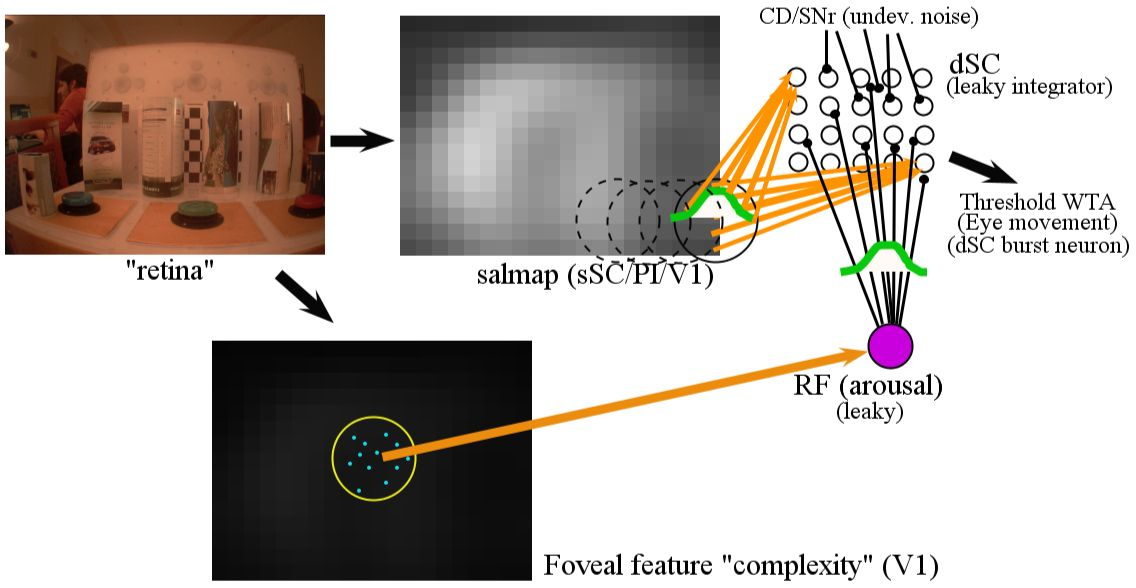
\includegraphics[width=15.0cm]{looking_prototype_model.jpg}
\caption{Graphical overview of connectivity and regions of network,
  and the general function of each region. Full-model anatomical
  correlates listed next to regions.}
\label{fig:looking_prototype_model}
\end{figure*}

The network is made up of several main pieces
(Figure~\ref{fig:looking_prototype_model}). The overall theory of its
functionality is illustrated in
Figure~\ref{fig:looking_functional_loop}.


\subsection{Saliency Map}
Images (frames) come in (actually, one from each eye, left and right)
and are put through a saliency map (\cite{itti_etal_1998}), which
assigns a salience value to each location in the image by looking for
areas of high global ``uniqueness'' at many spatial scales. This is
accomplished by applying filters at many scales in parallel to detect
feature channels such as motion, color, intensity, orientation, etc,
and then subtracting and subsampling between sequential spatial
scales, within channels. This is meant to represent some sort of
``fast scene processing'' salience, which does not care so much about
the content at visual locations so much as the ``salience'' of
locations especially in relation to the rest of the visual field. It
is imagined that this type of saliency map would be used in orienting
behavior, which is of course exactly what the looking behavior in this
paper is about. Some of the saliency channels (color, orientation) are
not ones that would be processed by the superficial layers of the
superior colliculus (SC)(mostly responds to movement), nor is there
evidence for (explicit) spatial scales even in V1, so it is not clear
where a salience map would actually be implemented, especially in an
infant.

\subsection{Superior Colliculus - deep (integration, eye control)}
The instantaneous salience map calculated for every frame is treated
as ``input'' into a longer-term map made up of leaky integrating
neurons (non-firing). This is considered to correspond to the
intermediate/deep layers of SC, especially since this is the last
``stop'' before eye movements in our model. Each neurons membrane
potential $V_m$ is described by the equation:
\begin{equation}
\frac{\partial V_m}{\partial t} = \frac{-(V_m - V_{rest}) + R_m \cdot
  (I_{bg} + I_{syn})}{\tau_m}
\end{equation}
where $R_m$ is the membrane resistance (uniformly 1.0 M$\Omega$ for
all neurons), $I_{bg}$ the background current (uniformly 0.0 mV for
all neurons) and $I_{syn}$ the total current impinging from afferent
synapses. The $-V_m$ represents the leakage term, causing the membrane
potential to decay exponentially with time constant $\tau_m$
(uniformly 30 ms for all neurons, though since update was per-frame
this has no relation to real-time). The resting potential of the
membrane $V_{rest}$ is assumed to be 0 mV.

Afferent input into a dSC neuron from the instantaneous saliency map
is simply linearly summed into $I_{syn}$, after being multiplied by
the efficacy of the synapse connecting it. The synaptic weights and
connections are built initially using a 2-dimensional gaussian, with
standard deviation $\omega_w$ (1.5 for the experiments) and a cutoff
value (i.e. minimum weight outside of which region there are no
connections) $\chi$ (0.05 for experiments). This has the effect of
slightly blurring (low-pass-filtering) the instantaneous salmap (thus
bringing out ``masses'' of high salience more than just isolated
pixels of high salience). It also mimics the increase in receptive
field size one sees when moving more towards the dSC (many
pre-synaptic neurons connect to fewer post-synaptic neurons, in
retinotopically defined areas).


\subsection{Reticular Formation (arousal response to complexity)}
%HR deceleration, Richards etc.

Physiological functions (arousal, measured by heart rate) have been
shown to be correlated with attentional phases in infants
\cite{richards_casey_1990}. Some have hypothesized the underlying
circuits for these include e.g. the reticular formation (RF) which is
responsible for the ascending transport of neuromodulators (horomones)
to diverse regions of the brain. Such areas could become more active
in response to stimulating environments (i.e. with more complex
stimuli, more variation, etc.) and are also responsible for the lack
of responsiveness of infants without sufficient stimulation. Though,
endogenous ebb and flow guide a large part of the very young infant's
arousal/attentional state at any time.

The complexity-responsive functionality of the RF circuits are used as
a mechanism for determining (soft) looking time towards an
object. Really, it could be implemented via other things such as
simply probabilistic microsaccades that are more likely to get
``caught'' in the more complex stimulus. Since usually the amount of
looking time towards a stimulus during e.g. habituation experiments is
postulated to be a function of ``encoding'' of the stimulus (and thus,
longer for more complex stimuli), yet we have explicitly lesioned
those areas that are ``making progress'' in any sense (or learning),
there must be some other mechanism than simply ``learning'' that
drives looking time towards stimuli. Since in habituation experiments
the salience etc. of stimuli is controlled, it is not easy to decouple
the habituation response from the ``baseline'' stimulus response. Note
also that more complex mechanisms, e.g. encoding into some sort of
short-term memory, waiting for a non-transient response/cycle of some
minimal error threshold in response to the stimulus, could be how this
stimulus complexity causes longer looking times, but the current
mechanism at least attempts to capture the phenomenon if not the
mechanism. This is perhaps one of the least understood areas of
oculomotor behavior -- namely, in absense of any scene change, what
causes the infant to look away? Several observations exist that
correlate with the phenomenon, e.g. the dying out of fixation neurons
in dSC, changes in activity in SNr, CD, and the buildup of burst
neurons in dSC, but the real dynamics and mechanisms and how all these
work together to move attention (fixation) are not well
understood. This is one of the things this model and the more
plausible one hope to offer explanations for.

In the model the RF is modeled as a single leaky neuron. One can think
of it as population coding of the activity of some region that got a
shot of neuromodulator/horomone cocktail in response to exciting
foveal stimuli. The RF neuron inhibits every region of the dSC, so
that more activation of the RF will result in more inhibition of SC
(pushing the neurons there to very negative potentials), and thus it
will take longer for SC neurons to recover via the normal continuous
input coming from e.g. the instantaneous saliency map and the gaussian
noise from SNr. However, to prevent the continuous fixation over
multiple ``refixations'' of the central area (which might not be coded
in mammals, i.e. we wouldn't have to worry about the currently
foveated area ever getting burst neurons activated since there are no
corresponding burst neurons there) the weighting of this inhibitory
projection is topologically modulated, such that more foveal/central
positions have stronger inhibitory weights than the periphery (which
still have some baseline inhibitory weight).

Thus, the weight of a point in the retinotopic projection as a
function of distance from the centre of the fovea is equal to the
value at that point of a gaussian centred on the centre, with
amplitude $\alpha$ (6.0), variance $\sigma$ (1.5), and baseline
(i.e. y-shift) $\beta$ (1.0).

When a gaze shift is made, the ``complexity'' $c_f$ of the current
foveal content is scaled and injected into the RF neuron (the RF
neuron's $V_m$ is set to $c_f$. In this case, as a standing, the
complexity is calculated as the number of Harris feature points
(thresholded 1-d gaussians LPFs run along the x- and y-dimensions)
within a radius $r$ of the centre of the image. In binocular cases the
two eyes are simply summed together linearly.

The RF neuron's membrane potential ($V_{RF}$) decays exponentially
with some time constant $\tau_{RF}$ (500ms, though again since in the
experiments update of the saliency model is not locked to real time
the units are arbitrary w.r.t. the experiments), i.e.
\begin{equation}
\frac{\partial V_{RF}}{\partial t} = \frac{-V_{RF}}{\tau_m}
\end{equation}

The membrane potential of RF is injected directly into all (e.g. dSC)
post-synaptic neurons, simply linearly scaled by the weight of the
synapse connecting RF with that neuron.

\subsection{Substantia Nigra pars reticulata (Gaussian noise)}
%because of e.g. unstable dynamics from dopamine...SNc...

Caudate Nucleus (CD) and SNr neurons show visual and habituation
responses \cite{hikosaka_wurtz_1983_SNr1}, which implies they are at
play in normal visual search behavior and/or habituation
learning. Assuming it's just habituation or even considering they are
engaged in disgengagement and thus normal visual looking behavior
(\cite{johnson_1990}), these disengagement and habituation behaviors
are not seen in infants or in limbic-cortex lesioned primates,
respectively. This suggests that the SNr itself, it's afferents, or
its efferents to dSC are undeveloped in the young infants. SNr-dSC
projections are known to be strongly GABAergic and thus inhibitory,
and to receive inhibitory projections from CD (``dis-inhibitory'',
which in turns gets input from a variety of regions as well as having
interesting intrinsic dynamics involving dopamine via SNc). We model
these dynamics and the product of immaturity by simply considering the
baseline of SC as already receiving some amount of inhibition from the
tonically firing SNr GABAergic neurons, and then add or sutract
gaussian noise (gaussian random variables) from the synaptic input to
each dSC neuron on every time step. The probability of drawing an
input of strength of $\delta$ is probabilistically based on the mass
of the gaussian at the point, thus small numbers are likely, and very
far out numbers are less likely. In the experiments, the noise is
drawn from a gaussian with $\sigma$ of 0.01 and amplitude (scale of
output inputs) of 1.0.

%2) OVERALL FUNCTIONALITY (i.e. rationale/mechanism of functioning to achieve desired behavior)
\begin{figure} [!t]
\centering
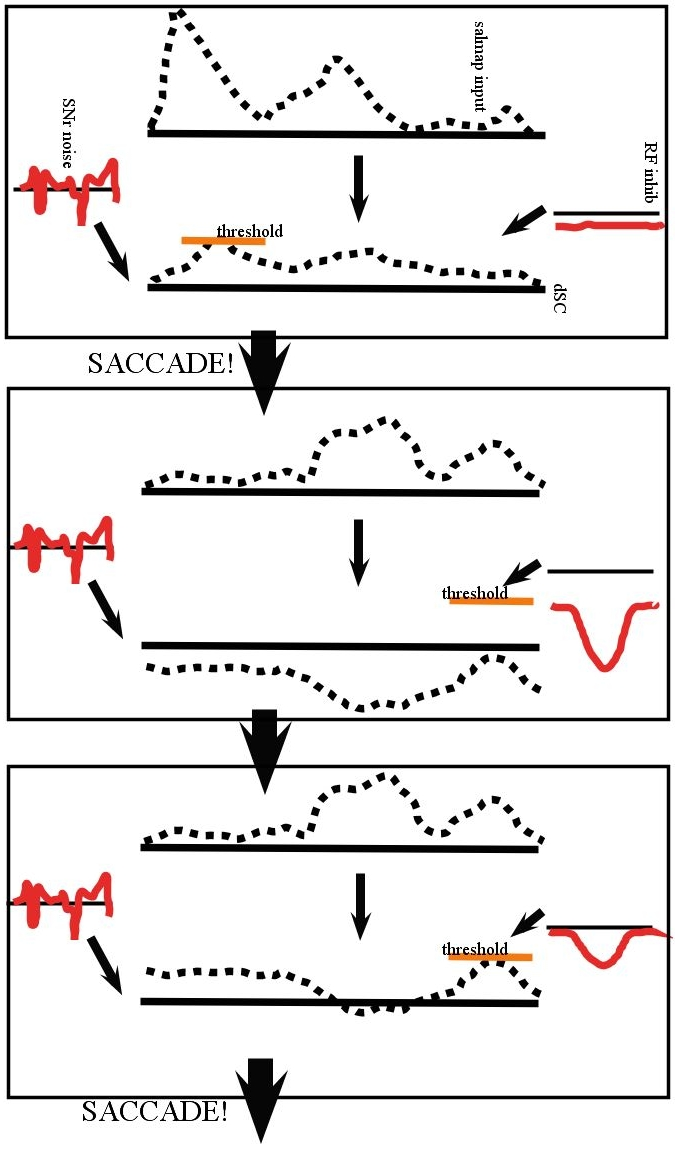
\includegraphics[width=6.0cm]{looking_functional_loop.jpg}
\caption{Intended loop dynamics of the model through several
  fixation-saccade iterations. Intended local circuit response
  properties listed where predictable.}
\label{fig:looking_functional_loop}
\end{figure}

\section{implementation on icub robotic platform}
The prototype model was implemented on iCub robot head
(Figure~\ref{fig:icub_head}). It has two pan-tilt-vergence eyes
mounted in the head supported by a yaw-pitch-twist neck (see
picture). It has 6 degrees of freedom(3 for the neck and 3 for the cameras).
We make use of stereo information to select the most salient point in the scene. The saliency maps from both the eyes are input to the decision module to select the single most salient point in the scene irrespective of which eye the saliency point comes from \cite{RichardWillInclude}. However, the saliency points only at the interest points in the scene are considered for choosing. \\
An interest point is a point in the image which has a well-defined position in image space that is rich in terms of local information content around it and is stable against the variations such as brightness, scale etc so that it is repeatable from frame to frame. It is not clear as to how much the ability to locate such interest points are pronounced in infants, however, studies show that V1 areas of visual cortex are sensitive to many simple features such as orientations at a very early age \cite{malsburg1973}. So one can consider such a possibility, to identify discriminant features, to exist in a growing infant which starts identifying and distinguishing objects.\\
In this work, we use Harris corner points as interest points. A corner point is defined as the intersection of two edges or as a point for which there are two dominant and different edge directions in a local neighborhood of the point. Corner point serves the characteristic of an interest point as it has a well-defined position and can be robustly detected. To determine a Harris corner point the autocorrelation matrix of the second derivative images over a small window around each point is calculated the two large eigenvalues are tested whether they are greater than a threshold.\\
Once the Harris corner points are calculated on the left and right images, we find the correspondence of these points between them (which is done as described later). Those points that don't have a matching point on the other image are removed. We then evaluate the value of saliency in a local region around remaining harris corner points on both the images. We use a gaussian kernel to get an average response of the saliency map around the harris points. We select the most salient point from these values and find its corresponding location on the other eye by its best matched feature. This location in the stereo vision is where icub's attention should be drawn towards (see figure \ref{fig:saliency_harris}).
\begin{figure} [!tbp]
\centering
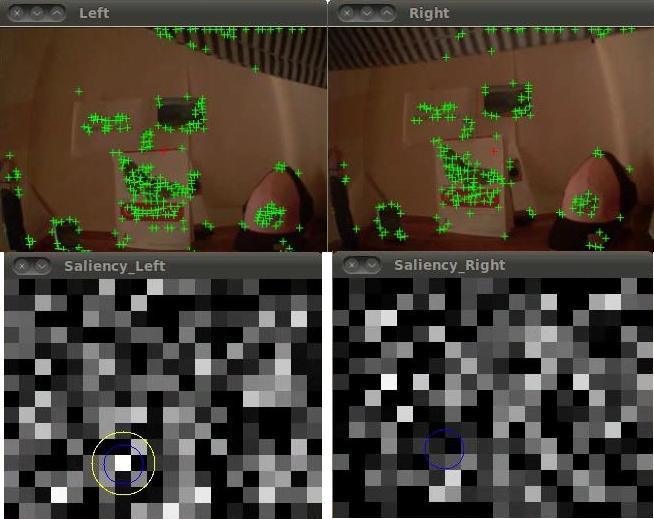
\includegraphics[width=8.0cm]{saliency_harris.jpg}
\caption{Saliency values at the Harris corner points are calculated and maximum of which is used to steer the attention}
\label{fig:saliency_harris}
\end{figure}
Next, iCub has to move its gaze towards the salient point and hence the object will be focussed in the center of the camera view. This task is accomplished using a tracking scheme that is completely object model free (Democratic Cue Integration \cite{triesch2001}). Democratic cue integration is a multi-cue tracking system that provides a fast and robust way to track unknown objects in a changing environment(lighting, background, noise, object motion). It combines information from various cues each with a weighting coefficient that depends on their agreement with all other cues. This makes the system adaptive to a given situation as the cues that are not suitable quickly lose the prominence. In our work we use motion, kalman prediction, template matching, color kernel tracking and contrast based kernel as different cues. \\
Tracking executed in the above manner provides a very robust coordinated movement of the head and eyes that is usually a challenging problem especially in binocular vision. One can observe that the movements accomplished by this way of a vergence-control
mechanism runs in a closed-loop fashion with visual input. It is not clear
how the problem of vergence is solved in infants but it seems to be clear that
saccades are not closed loop or vision-driven but are ballistic and
motor-driven~\cite{hainline_1998}. Since the model was turned off
during ``saccades'' this had no effect on the collected data, though
from a real-time point of view it was very slow compared with actual
saccades (limitations of the motors). Coordinated movement of the head
and eyes is likewise probably unrealistic in such young infants. \\
% However, the algorithm that we used helps us in tracking the first impression of the object at the salient point quite successively in spite of movement of the objects in the scene. This may explain the behavior of a growing child whose attention is quite pronounced and more object specific as learning is coupled with of their behavior(NOT SURE AGAIN!). \\
In the next step, we use stereo disparity information to coarsely segment the focussed object from the background. We calculate the stereo disparity at all interest points in the scene. To do this we calculate Gabor-jets at interest points on both left and right images. We then compare jets at all interest points in the left image with all points on the right image and we choose the best matching pairs of points by seeing the similarity between the jets (inner product between the vectors should be above a threshold value of 0.93). We then calculate the stereo disparity(horizontal as well as vertical) for each matching pair. The disparity of the interest points falling on the object that has been focussed is considered as the reference value and the points that are away from this value (more than 2 in both +ve and -ve directions) are considered to be from the other objects or background and hence removed. This procedure gives us a rough segmentation of the object or at least segregates the interest points (and hence the feature points i.e. gabor jets) belonging to the object from the rest (see figure \ref{fig:matching}. This would be helpful for initiating a learning process of the object. Finally, when the robot looks at the object, the time spent in looking at the object is made dependent on the complexity of the object (in our experiment, it is made dependent on the number of Harris corner points as already discussed in the previous section). The trajectory (i.e. ordering) of looking among the objects is recorded.
\begin{figure} [!tbp]
\centering
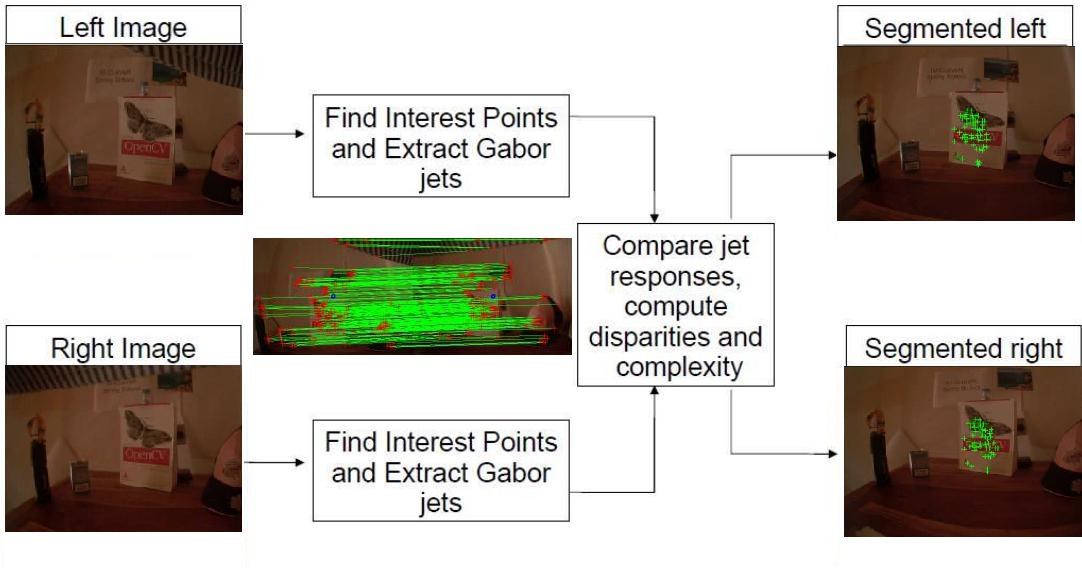
\includegraphics[width=8.0cm]{matching1.jpg}
\caption{Stereo segmentation by matching Gabor-jets at the interest points on left and right camera images.}
\label{fig:matching}
\end{figure}


%PICTURE icub
\begin{figure} [!t]
\centering
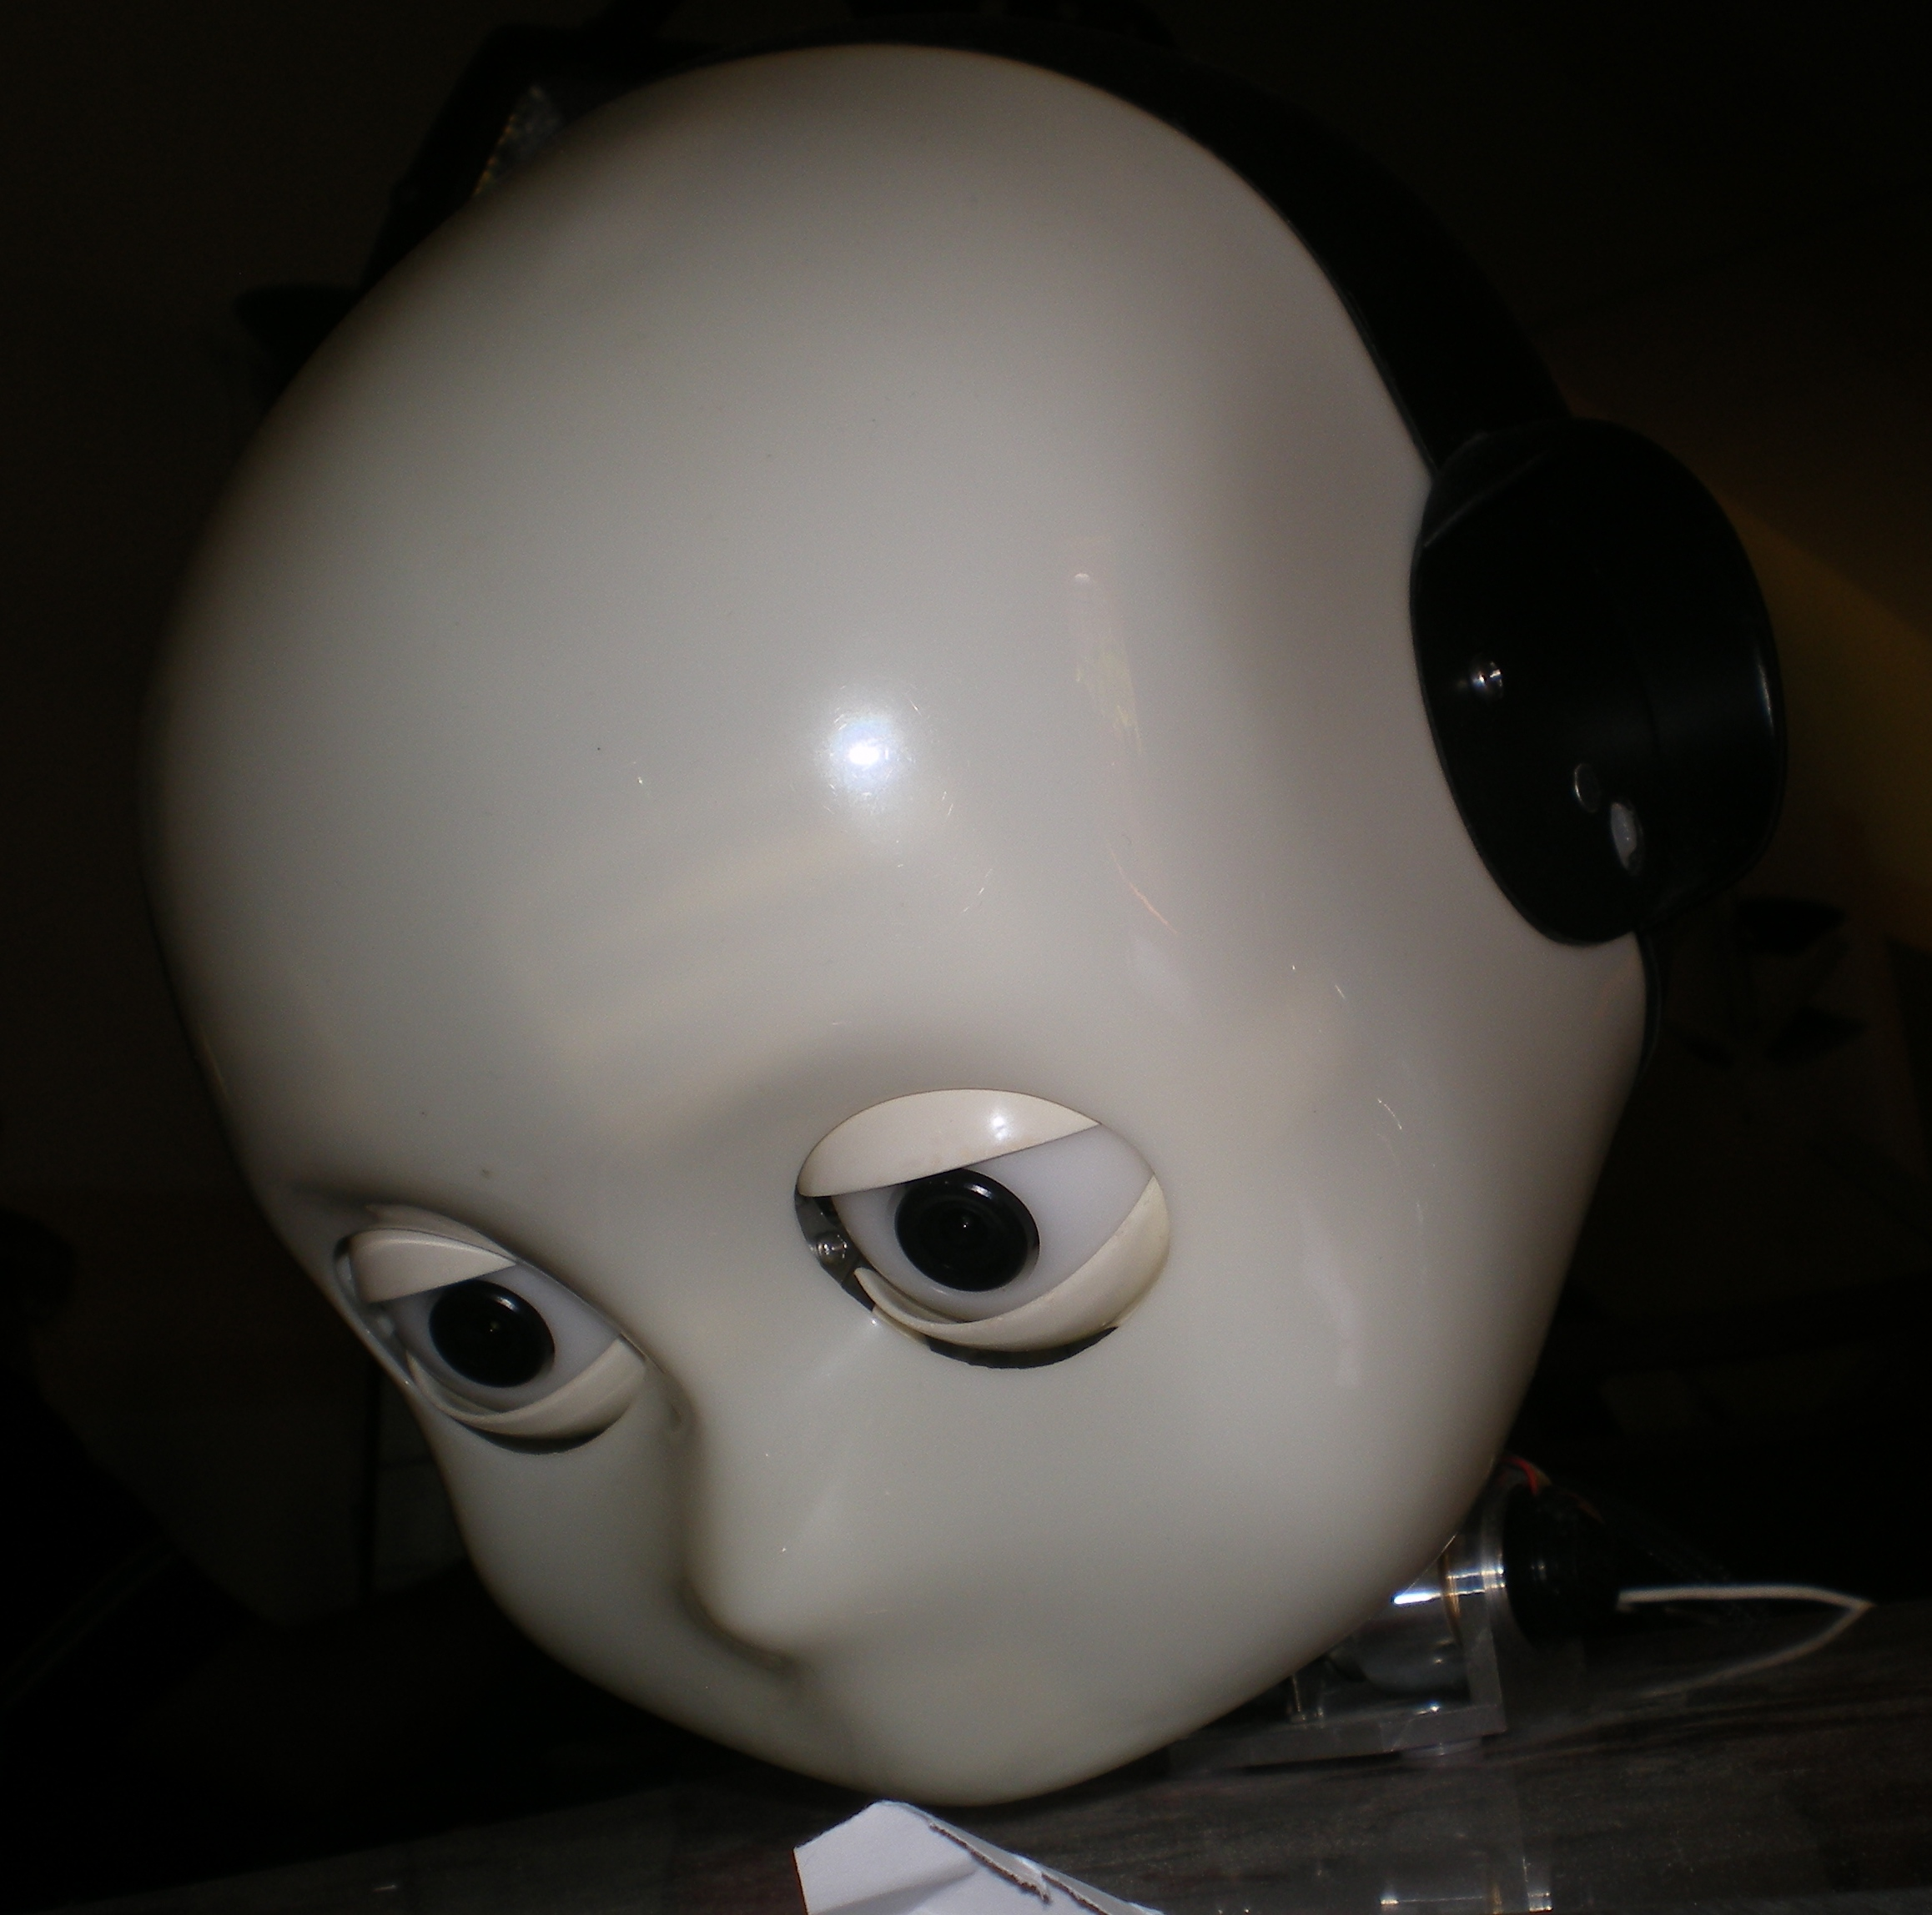
\includegraphics[width=3.0cm]{icub_head.jpg}
\caption{The iCub head that was used for the experiments.}
\label{fig:icub_head}
\end{figure}

%The robot instantiated the network and was placed in front of a scene. The amount of time spent looking at objects and the ``complexity'' of the object was recorded. The trajectory (i.e. ordering) of looking among the objects was recorded.

%PICTURE exp setup (example environ) also mention movement type thing?
%PICTURE icub
\begin{figure} [!t]
\centering
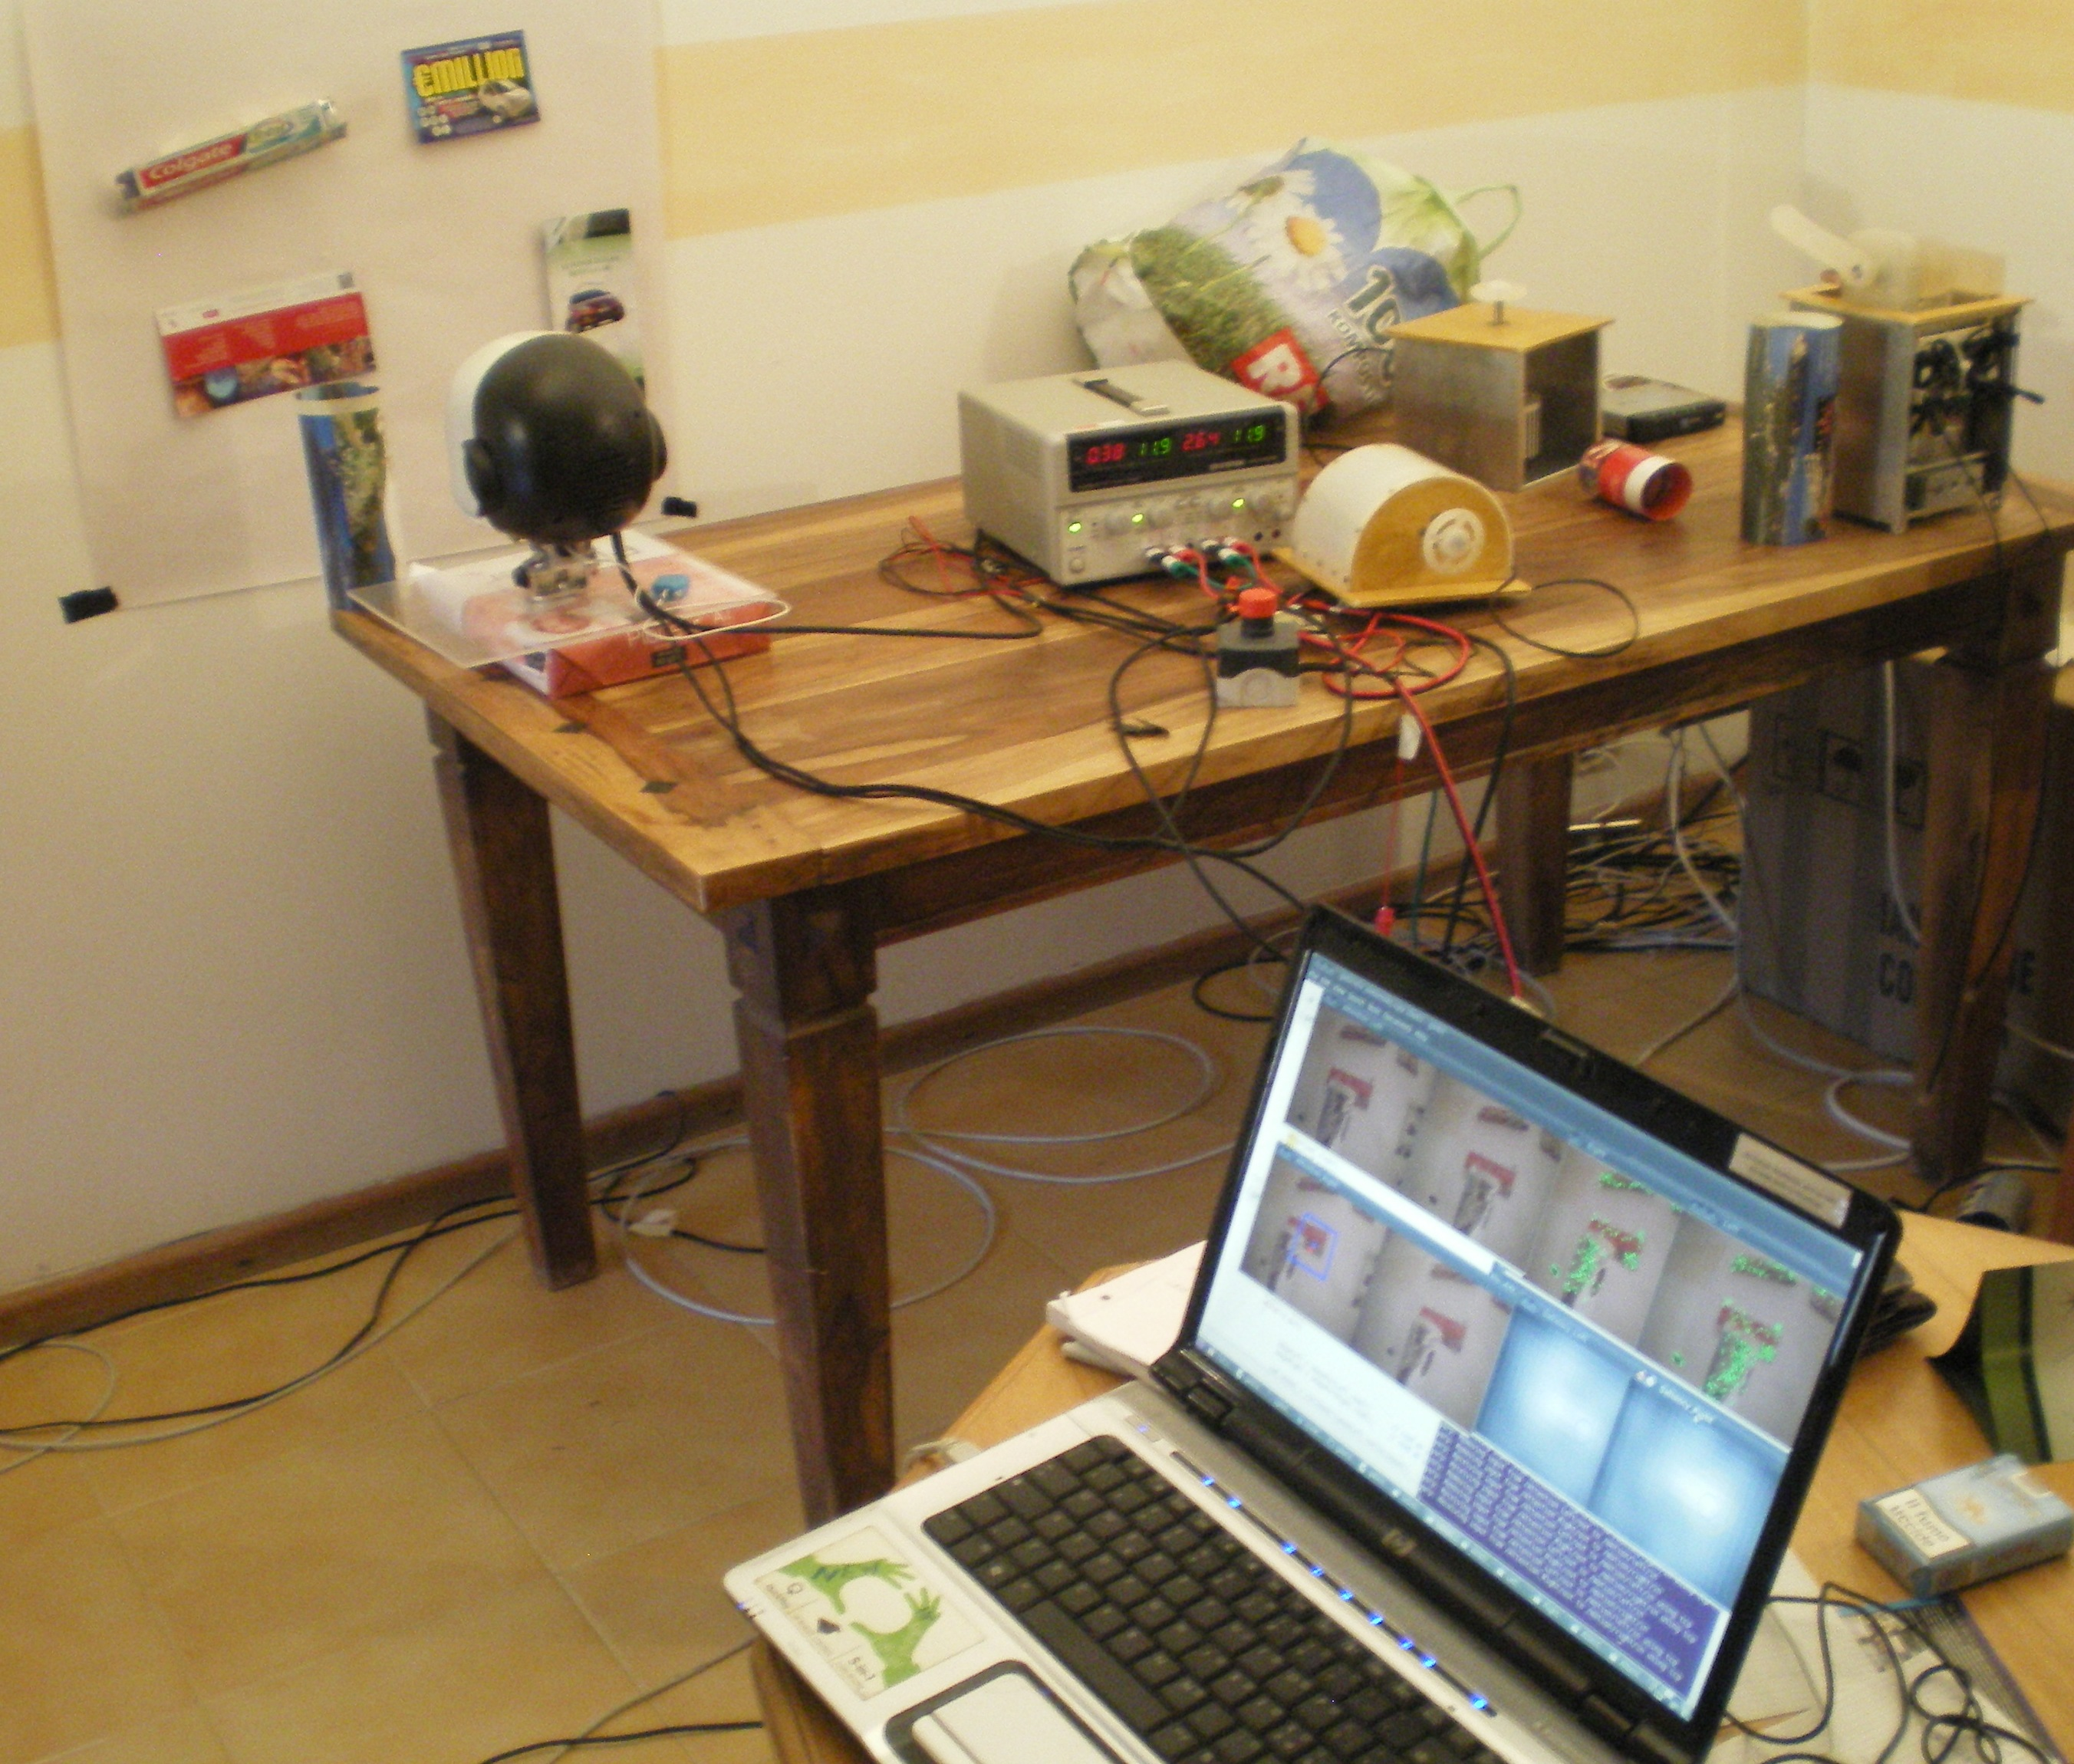
\includegraphics[width=6.0cm]{icub_setup.jpg}
\caption{A picture of the experimental setup that was used during the
  experiments. The type of environment presented can be seen in front
  of the iCub head in the upper-left corner.}
\label{fig:icub_setup}
\end{figure}

%********************RESULTS******************%
\subsection{Results}
Results will go here... Based on runs on single frames (see
testonppm.cpp) the decaying-inhibition dynamics of the model work as
intended. To demonstrate this, see
Figure~\ref{fig:complex_vs_fixtime}, plotting the results of automated
experiments with the model measuring the time between first fixation
and second fixation as a function of the complexity of the foveal
image (x-axis).
\begin{figure} [!t]
\centering
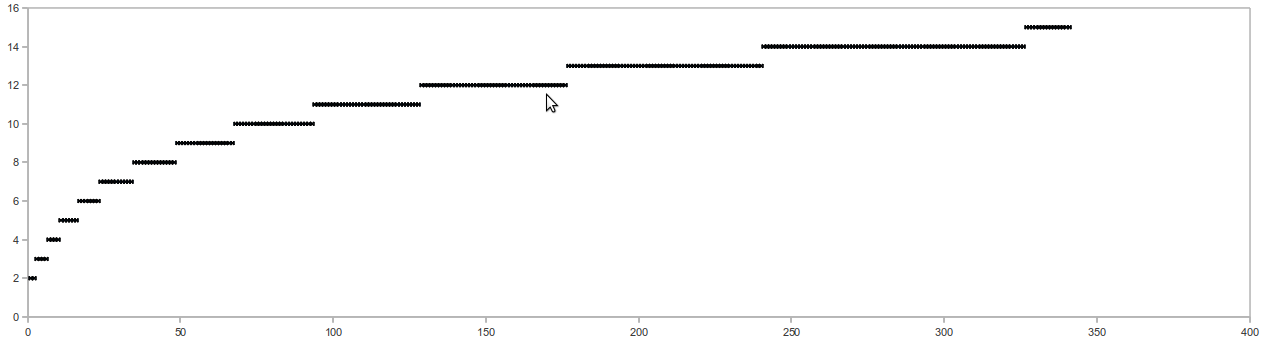
\includegraphics[width=15.0cm]{complex_vs_fixtime.png}
\caption{Plot of the time between fixations (i.e. fixation time to
  that foveal region) for varying levels of foveal complexity (the
  manipulated variable in these experiments). Note the logarithmic
  pattern that emerges: for very low complexities, fixation is
  disengaged quickly, and for slightly different complexities the
  looking time differs, but as complexity increases, the looking time
  saturates to a maximum.}
\label{fig:complex_vs_fixtime}
\end{figure}

This is the desired behavior, and would result in (at least) fixation
times that follow the desired model of fixation time. For the
longer-term looking dynamics, however, since foveation of the salient
stimulus is assumed, it's impossible to test the looking dynamics
without running on the robot or in a simulation environment that moves
the visual field.

\section{Conclusion}
By design, the mechanism to determine looking time towards a foveal
stimulus as a function of its complexity was successful, but this is
not the interesting result since these dynamics are predicted and
necessitated by the simple mechanism.

The interesting bit will be the inter-object looking behavior in a
real environment. Will, and how often will, the system make saccades
to ``noise'' areas but then quickly look away because of lack of
complexity?

In the future, the model will be implemented as the more complex
anatomical circuit, the saliency map replaced with proper neural code
from the eye-up, and the actual neurons ``fudged'' in most of the
areas and their dynamics actually simulated. The benefit of building
the more realistic model will be to actually look at the different
dynamics of the model in reaction to the changing environment, since
that kind of interaction can not be easily predicted or simulated.

%\bibliographystyle{apacite} \bibliography{bib}
\bibliographystyle{IEEEtran}
\bibliography{bib}

\end{document}
